	\begin{figure}[tb]
		\centering
		Priloha 1\\
		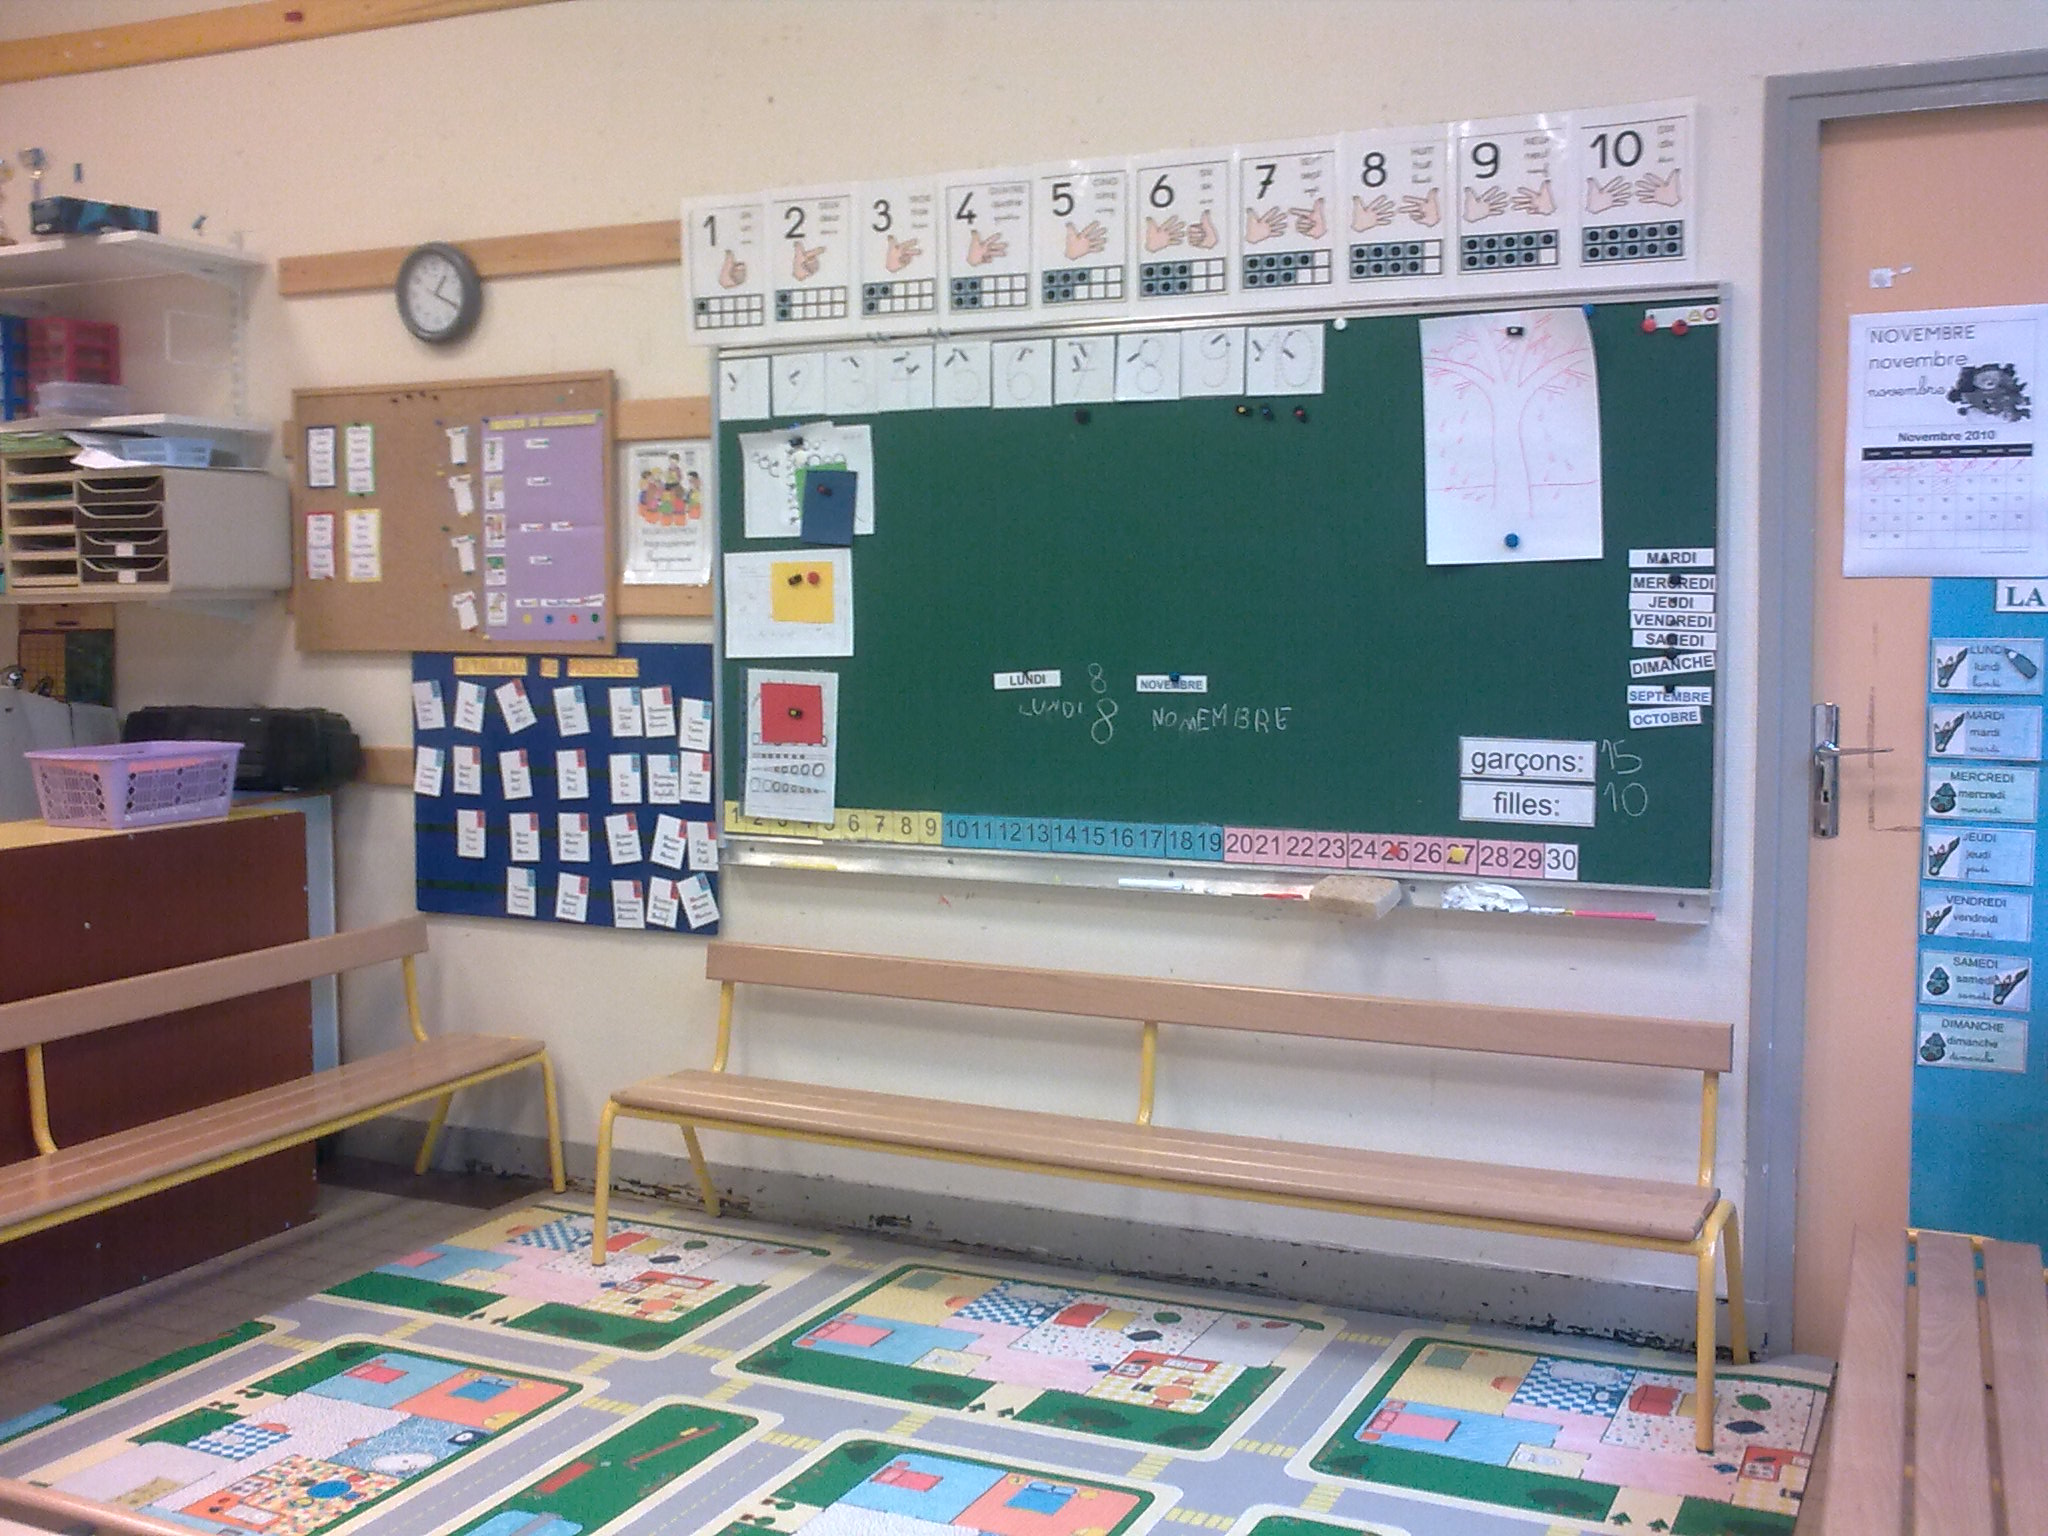
\includegraphics[height = 0.35\textheight]{./fotky/Obr1.jpg}
		\caption{
			Tabule s návody, číslicemi, datem a popisem dílen, prostor pro ranní kruh (viz.~\ref{tridaVybaveni}).
		}
		\label{Obr1}
	\end{figure}

	\begin{figure}[tb]
		\centering
		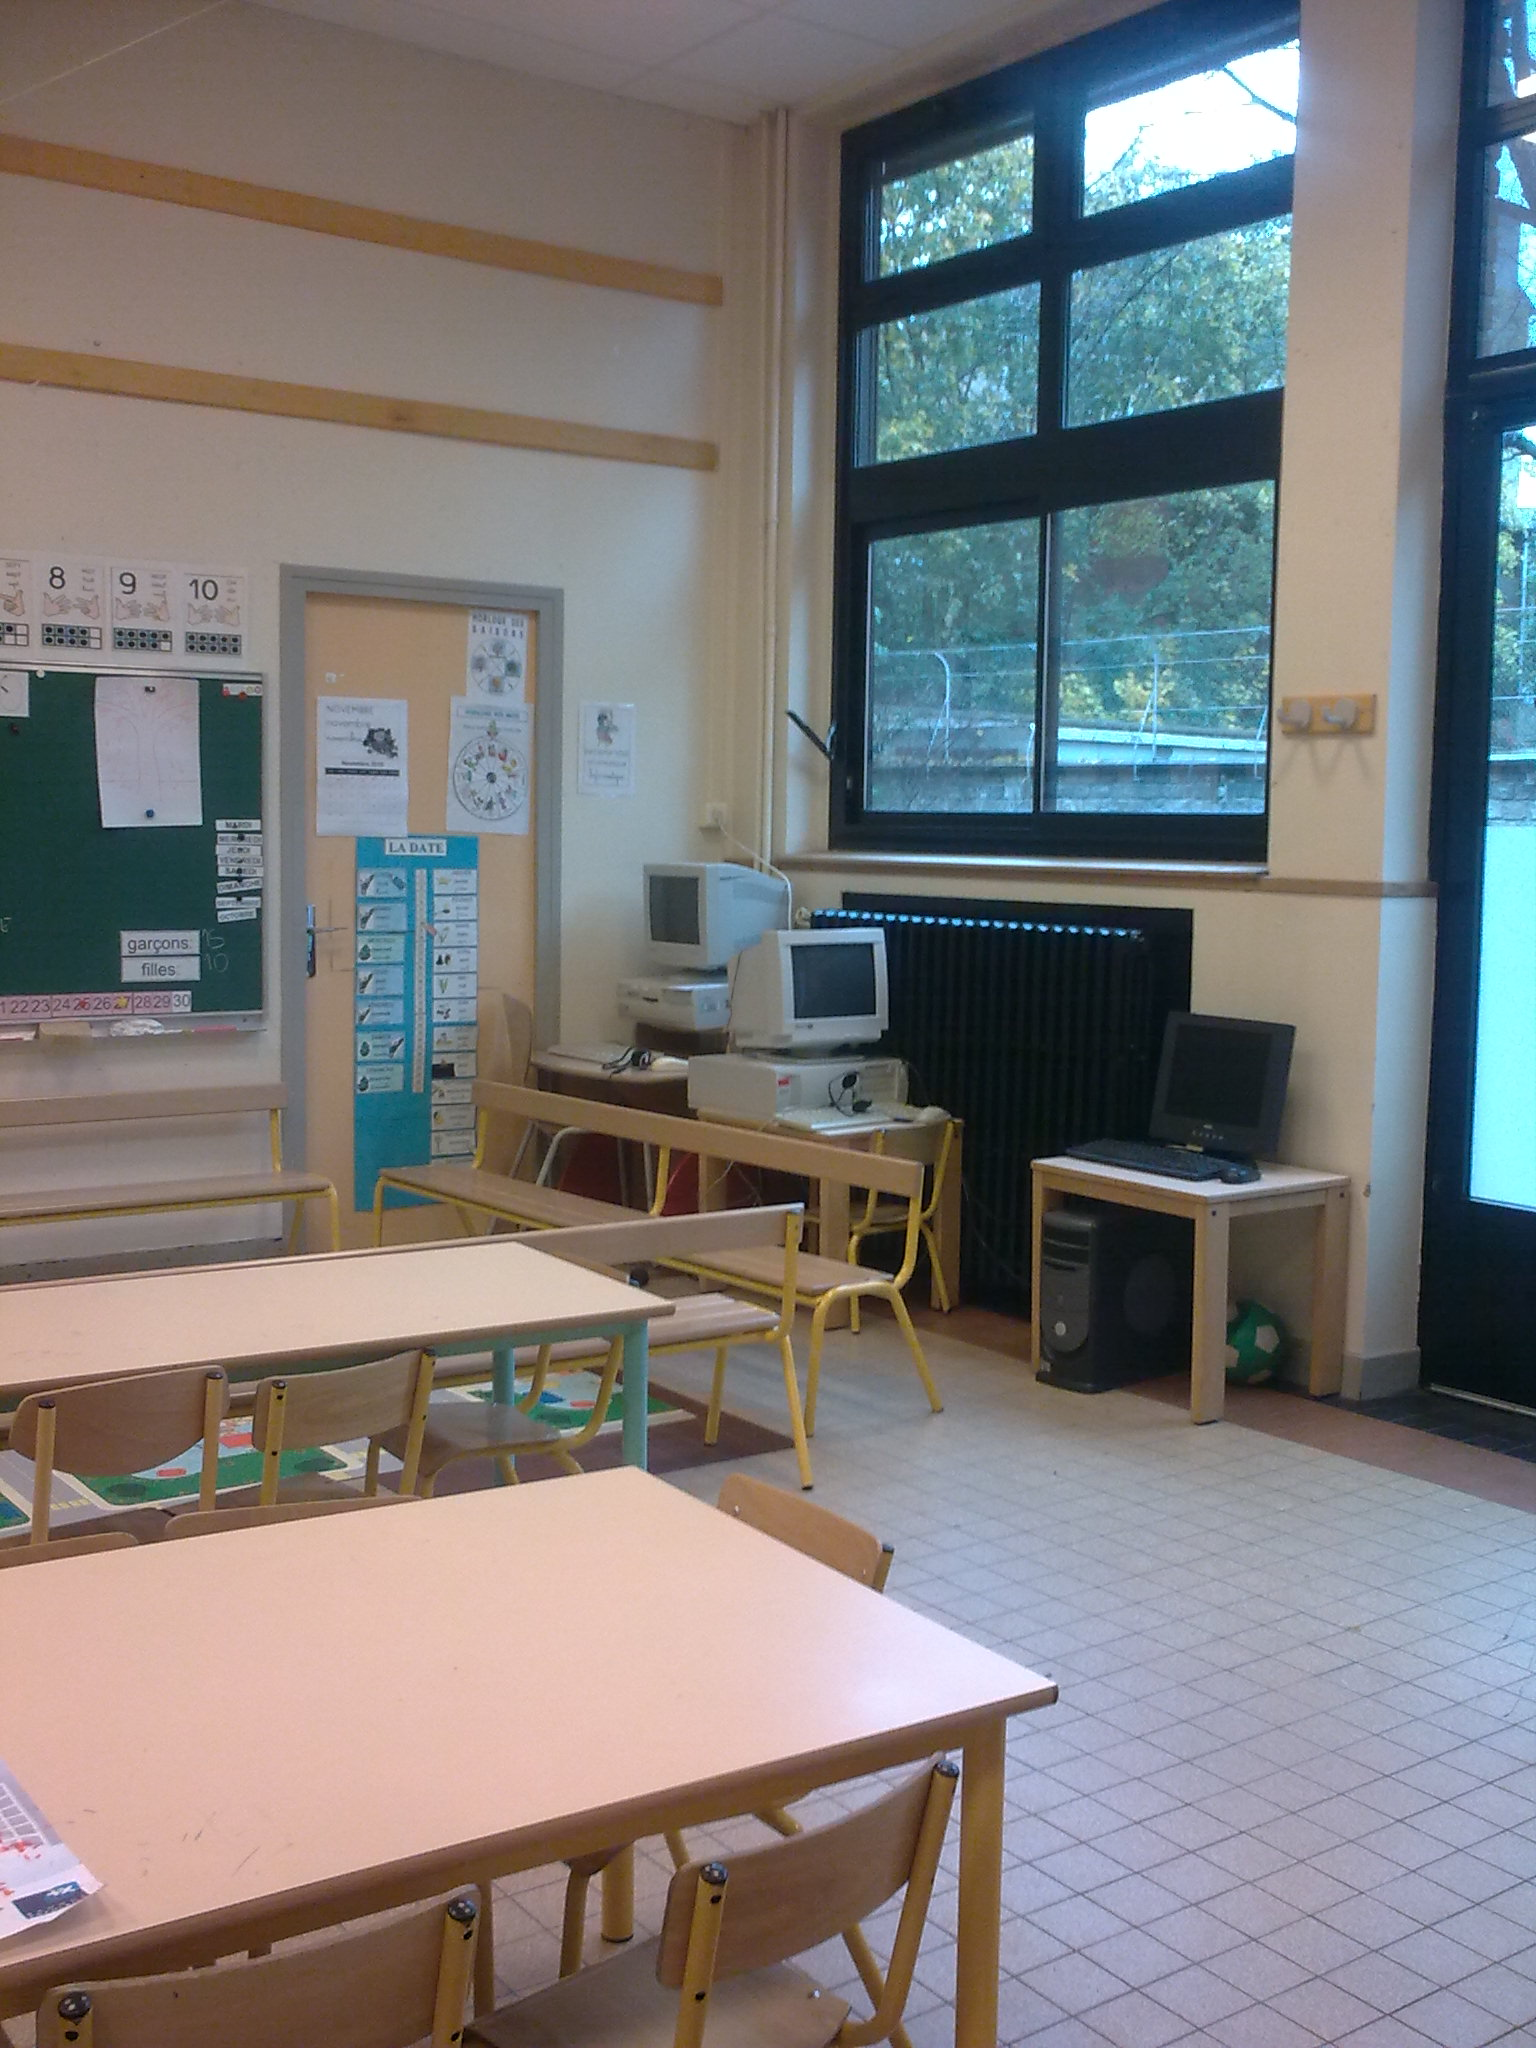
\includegraphics[height = 0.35\textheight]{./fotky/Obr2.jpg}
		\caption{
			Stolky s počítači a vchod na dvůr (viz.~\ref{tridaVybaveni}).
		}
		\label{Obr2}
	\end{figure}

	\begin{figure}[tb]
		\centering
		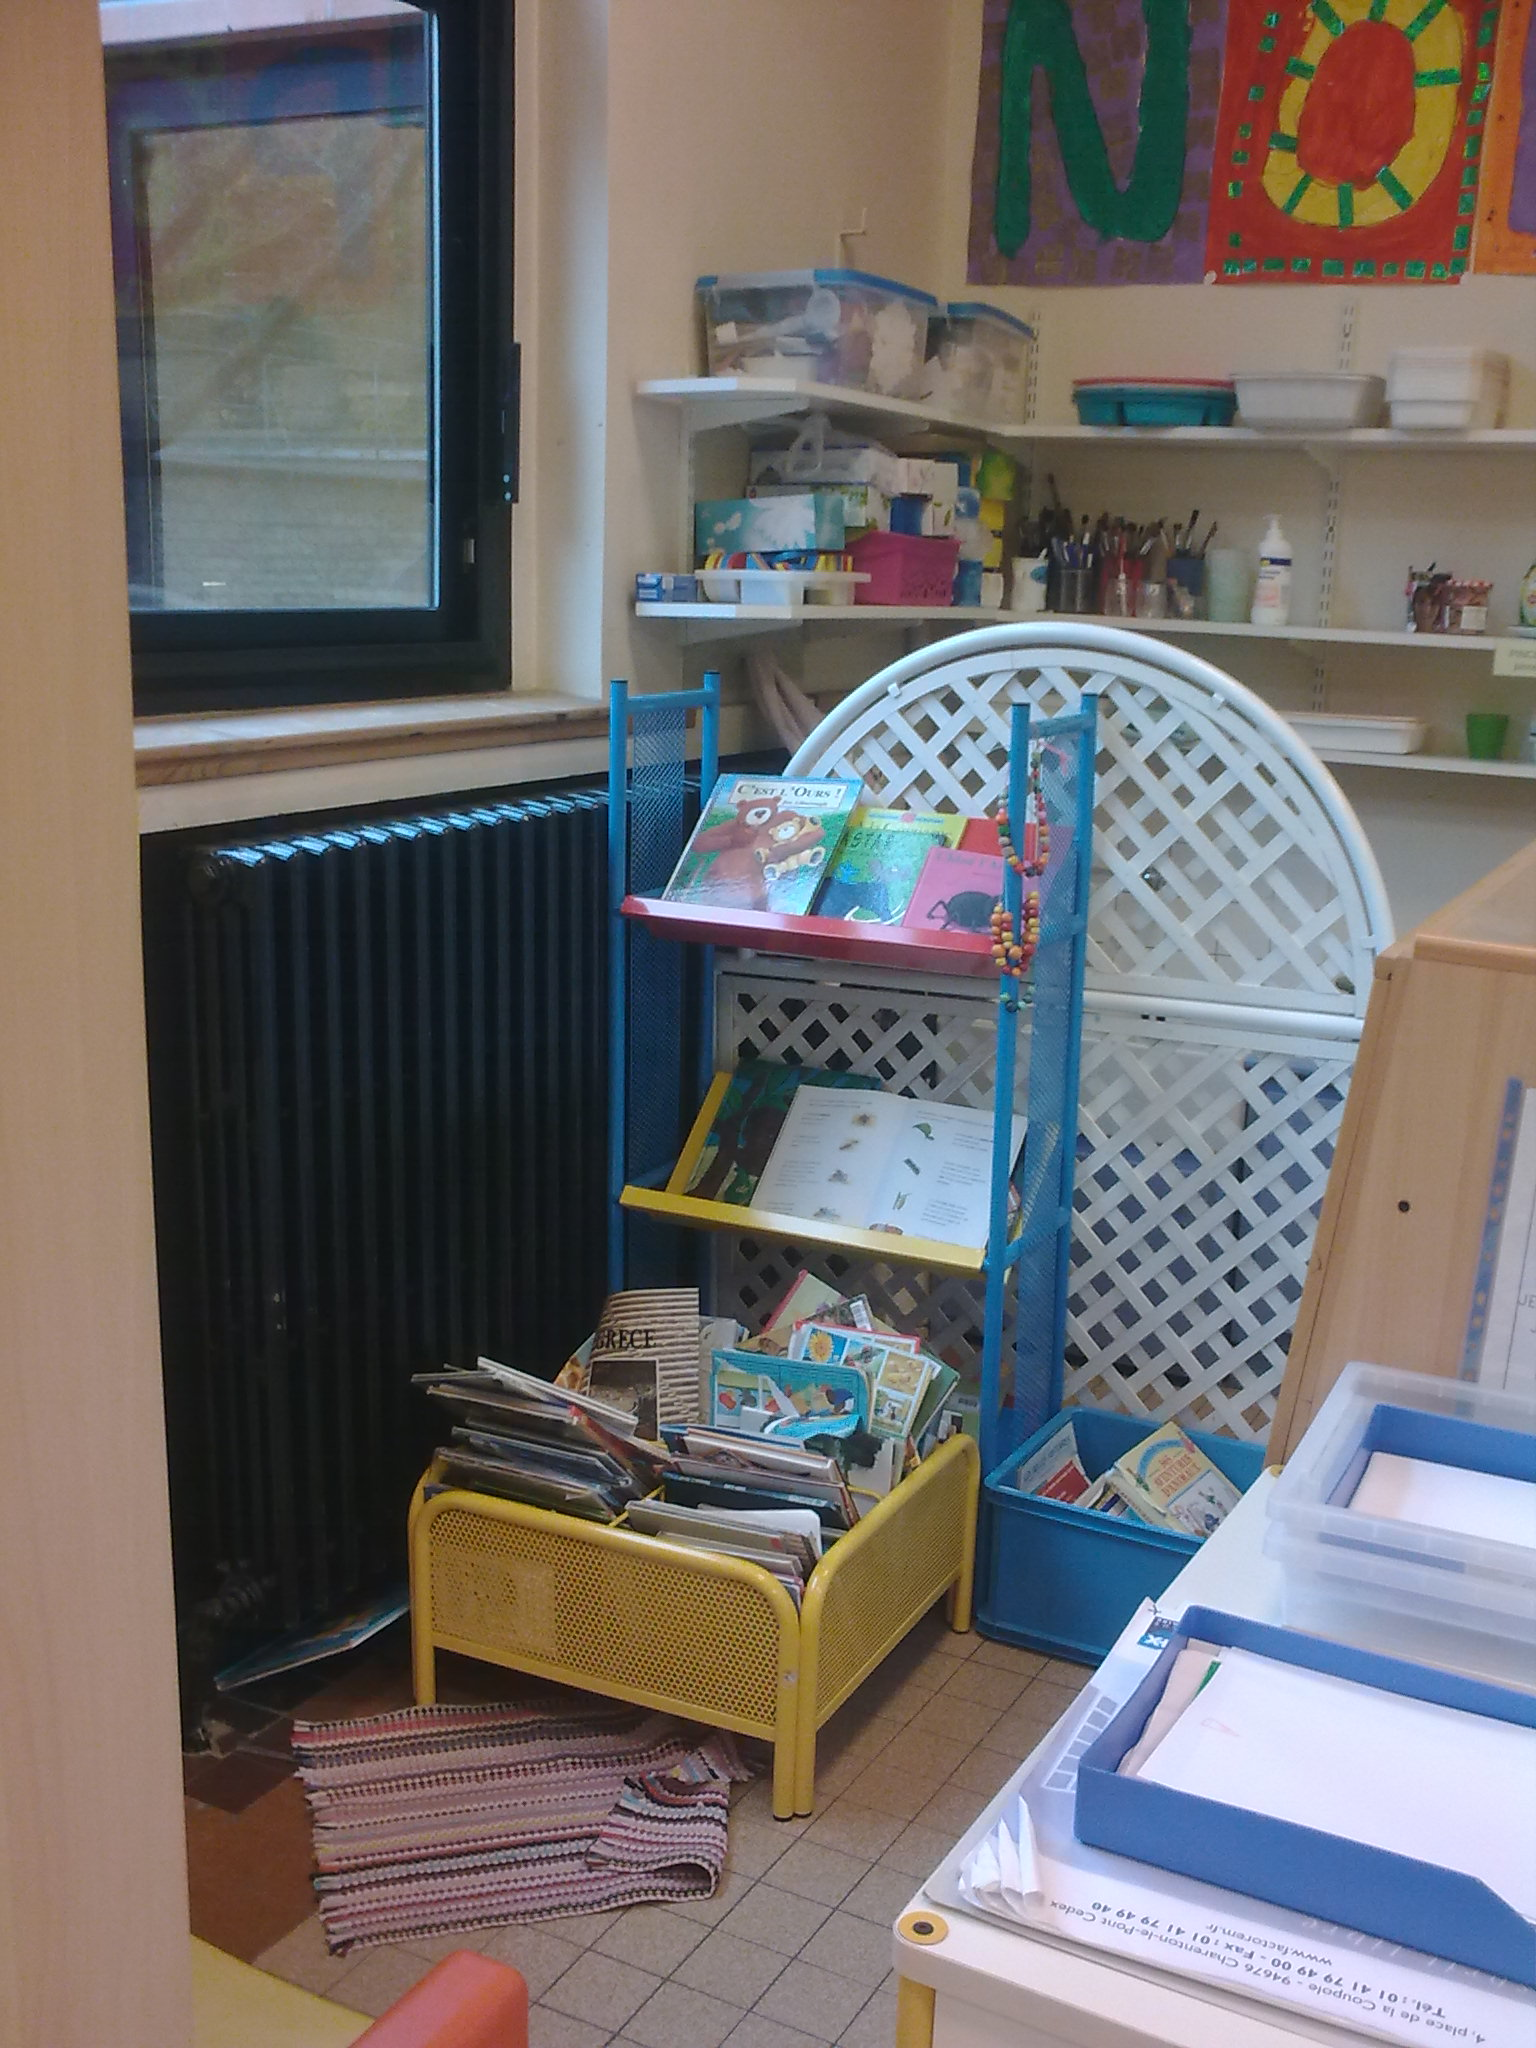
\includegraphics[height = 0.35\textheight]{./fotky/Obr3.jpg}
		\caption{
			Literární koutek s křesílkem (viz.~\ref{tridaVybaveni}).
		}
		\label{Obr3}
	\end{figure}

	\begin{figure}[tb]
		\centering
		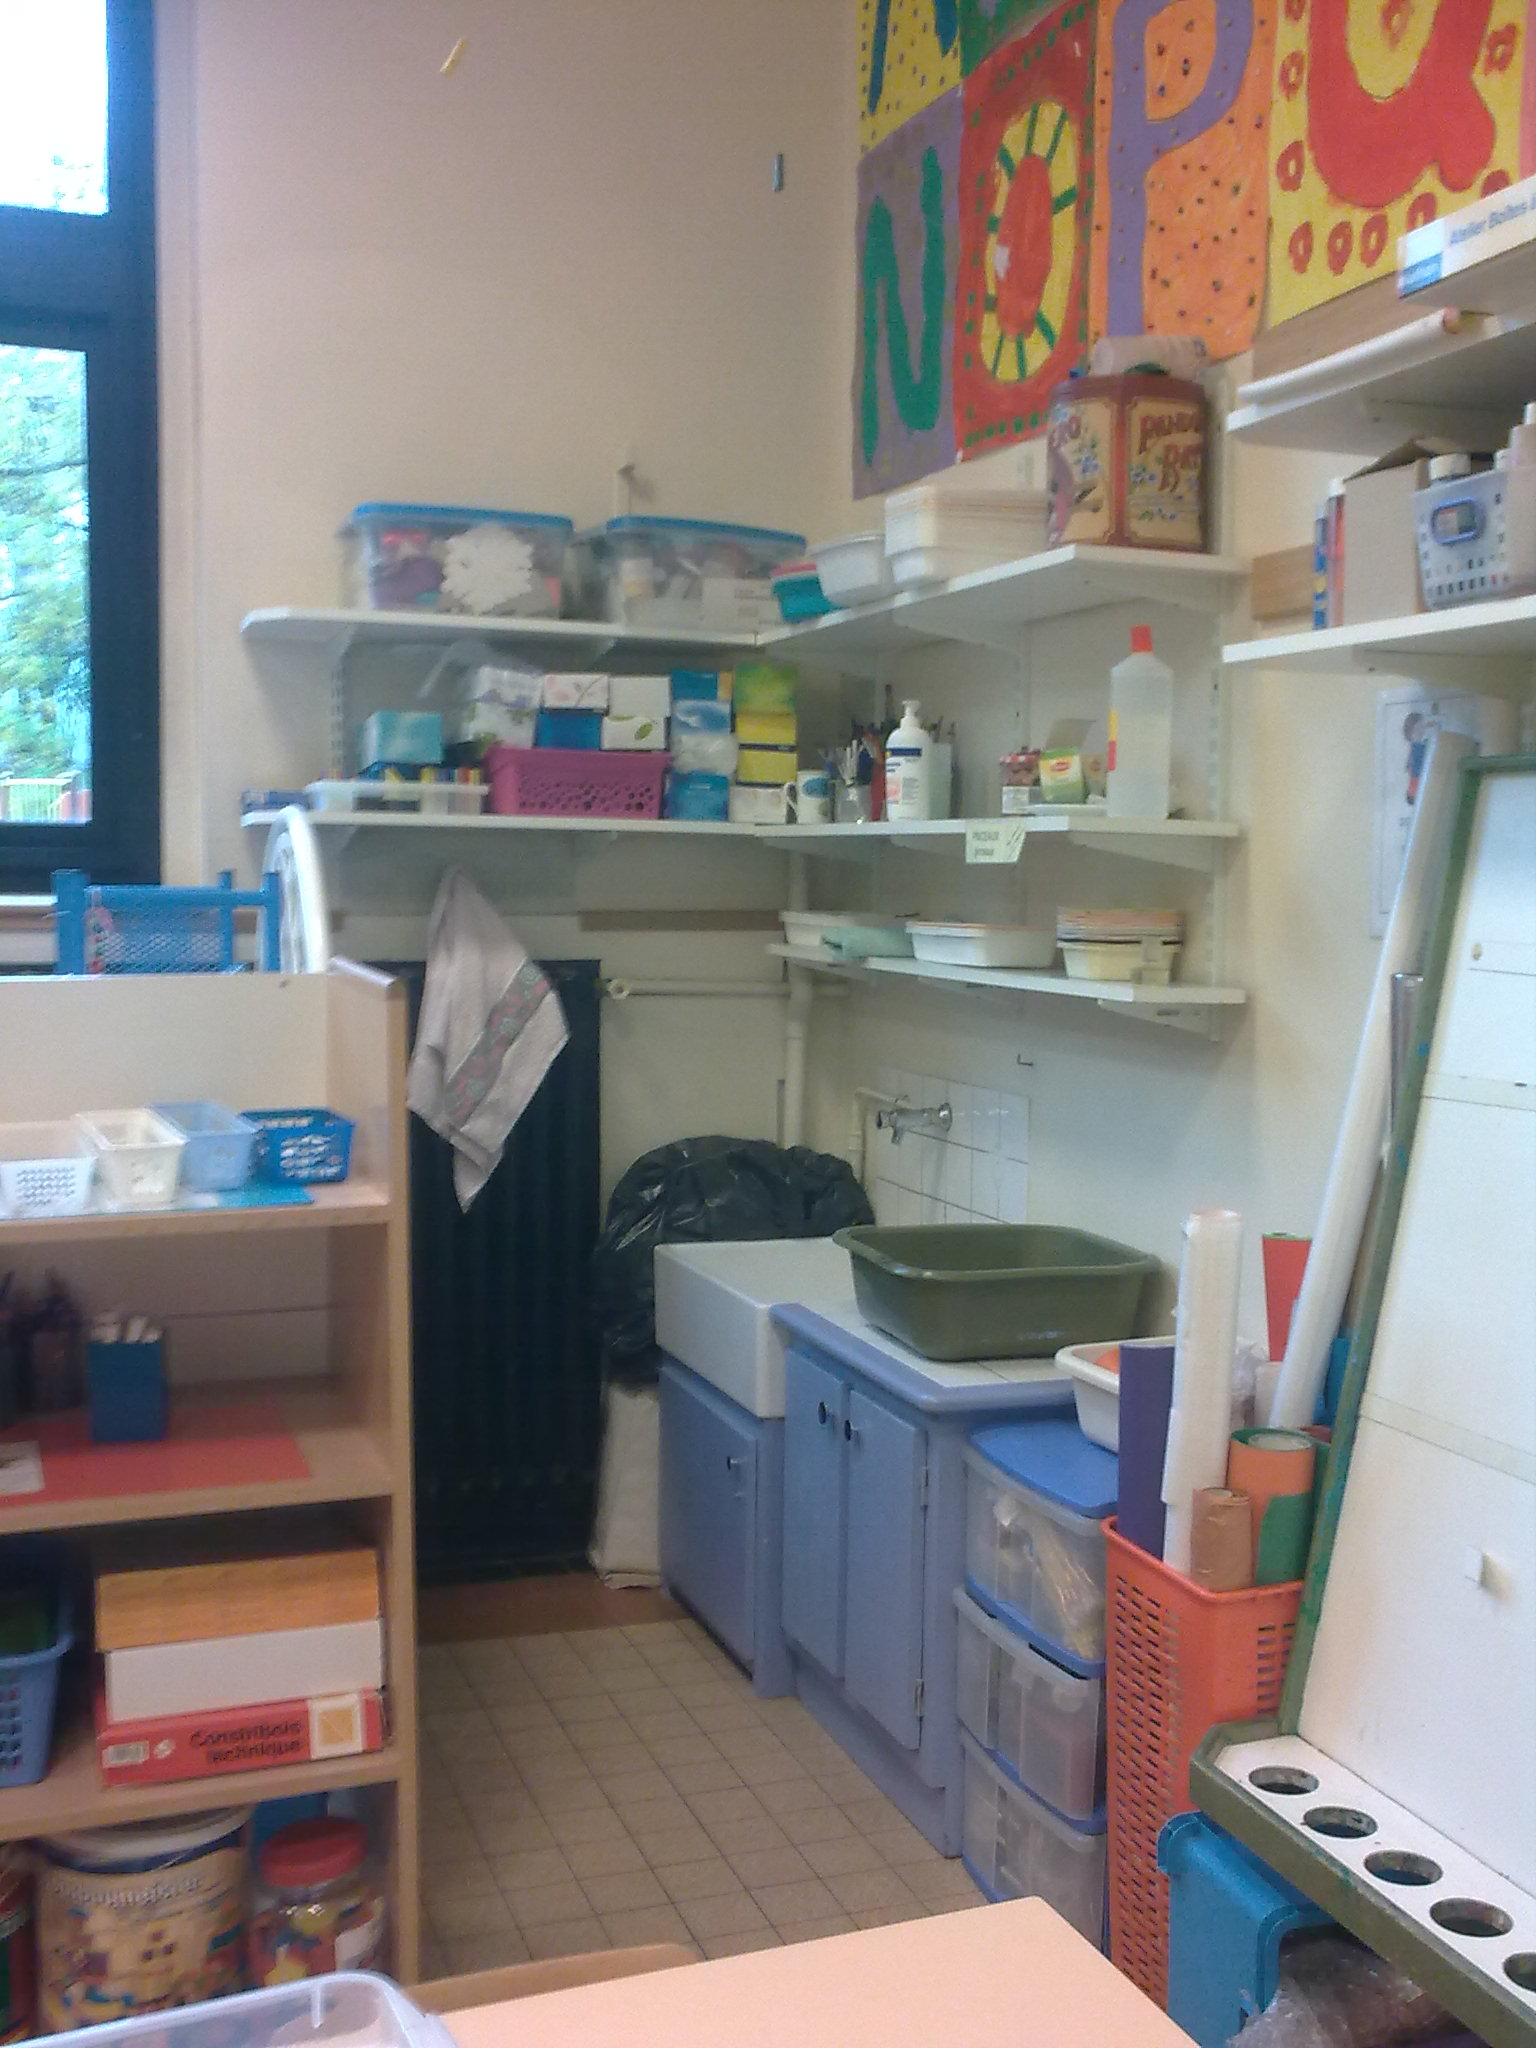
\includegraphics[height = 0.35\textheight]{./fotky/Obr4.jpg}
		\caption{
			Umyvadlo a police na materiál (viz.~\ref{tridaVybaveni}).
		}
		\label{Obr4}
	\end{figure}

	\begin{figure}[tb]
		\centering
		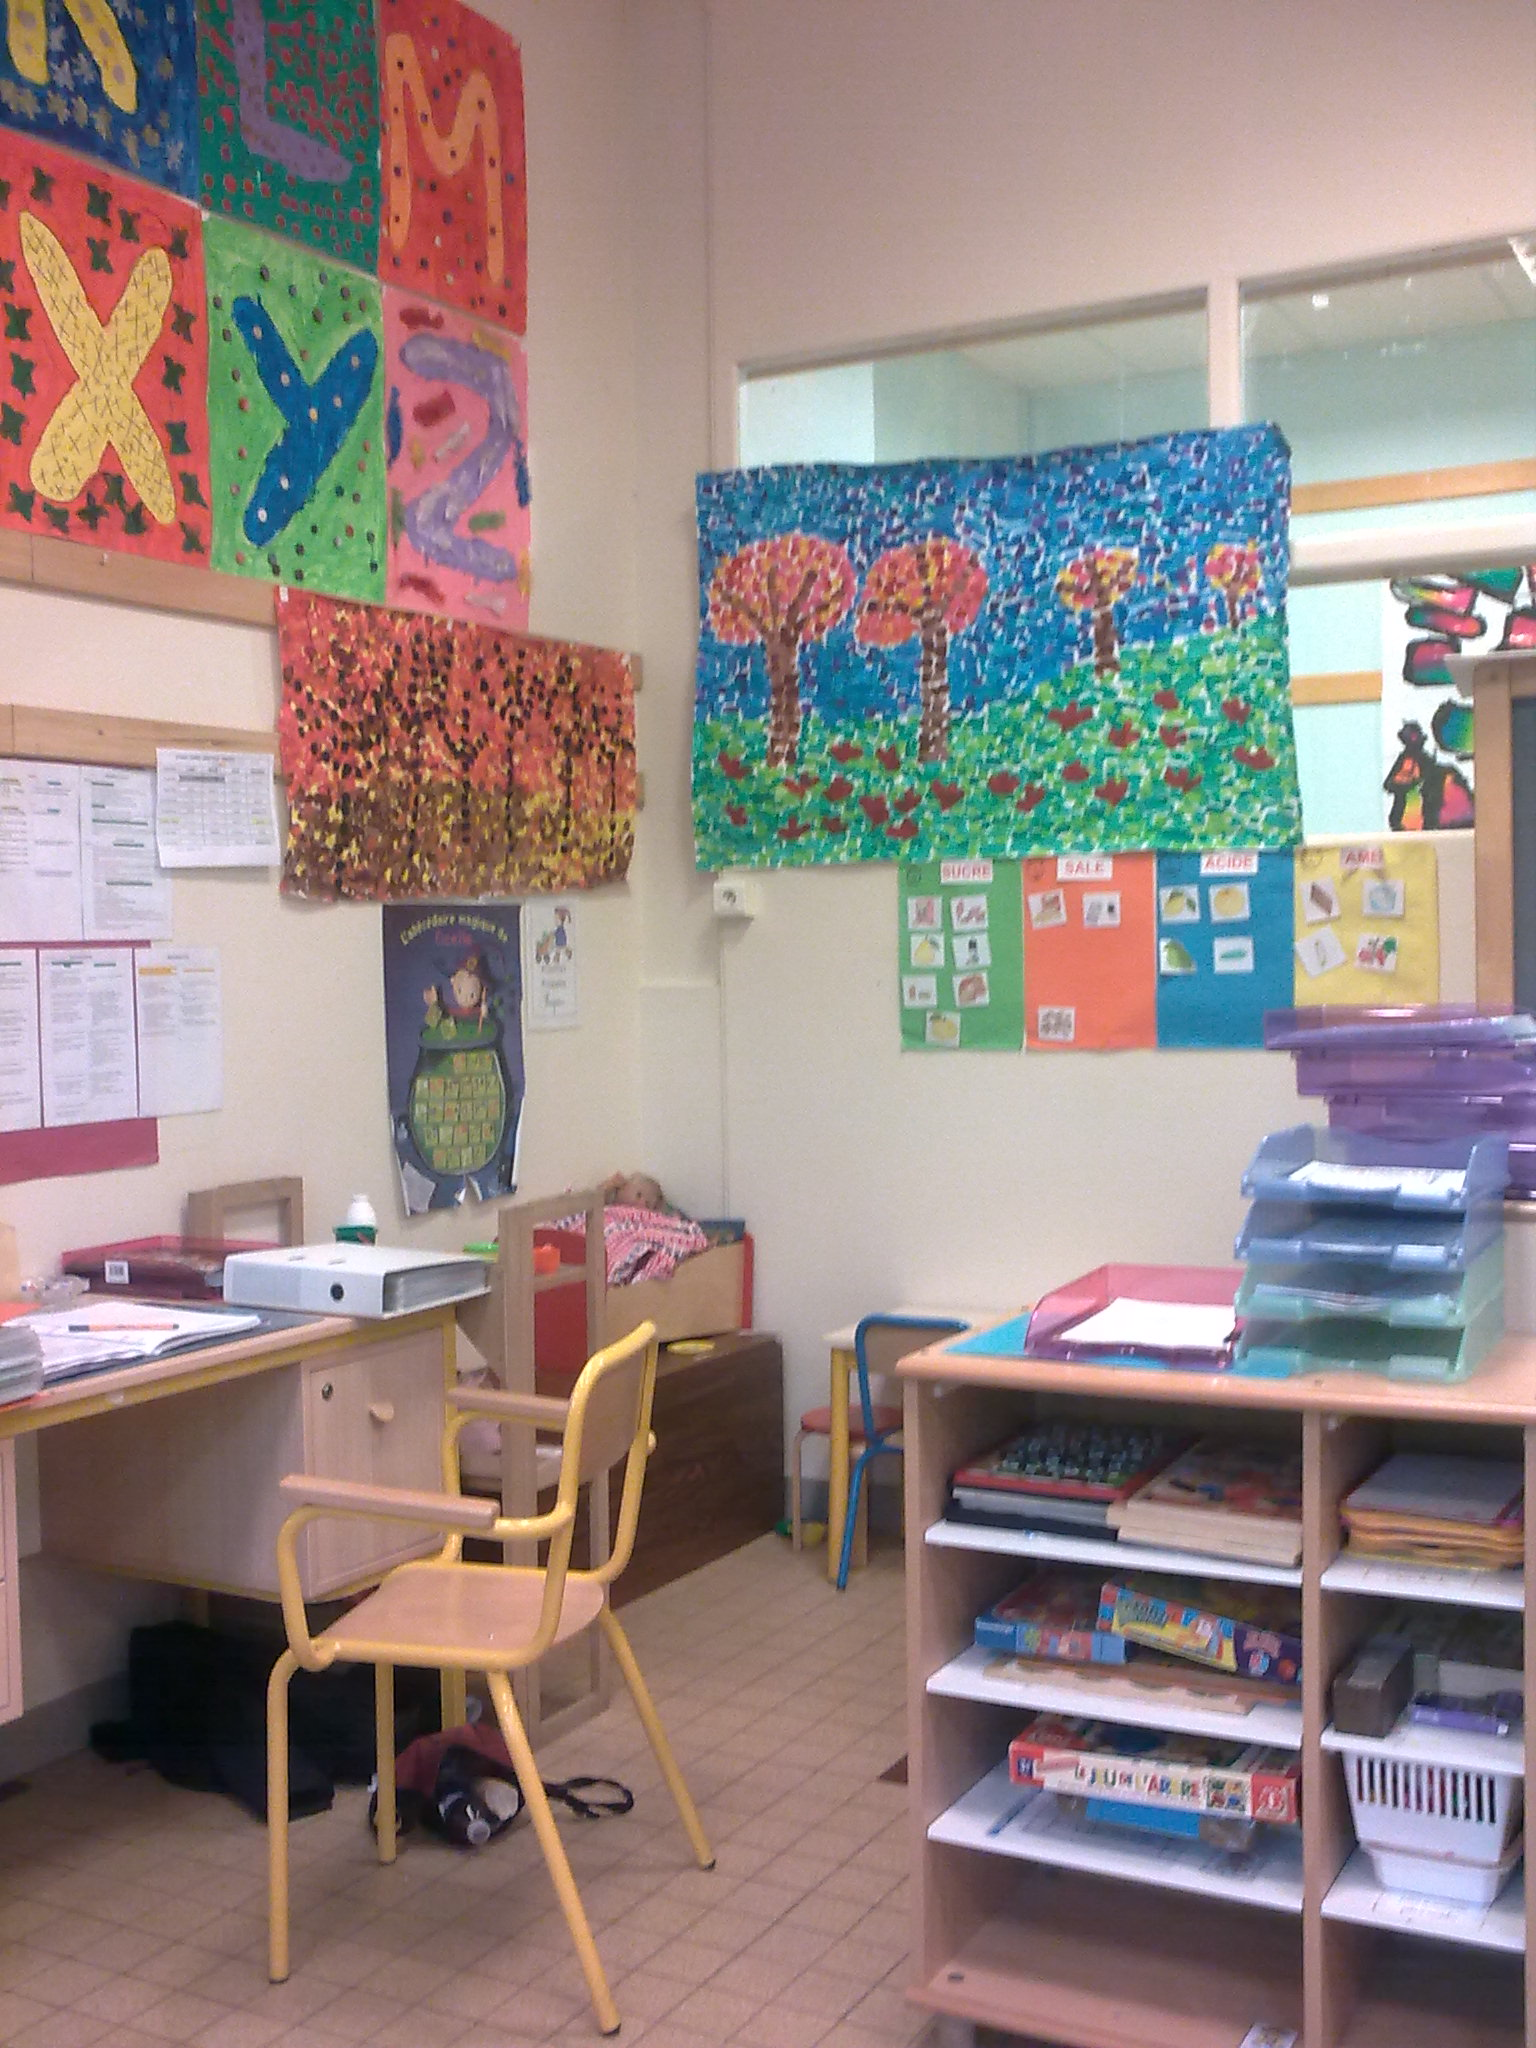
\includegraphics[height = 0.35\textheight]{./fotky/Obr5.jpg}
		\caption{
			Stůl pro učitelku, dětská kuchyňka a poličky na didaktické pomůcky (viz.~\ref{tridaVybaveni}).
		}
		\label{Obr5}
	\end{figure}

	\begin{figure}[tb]
		\centering
		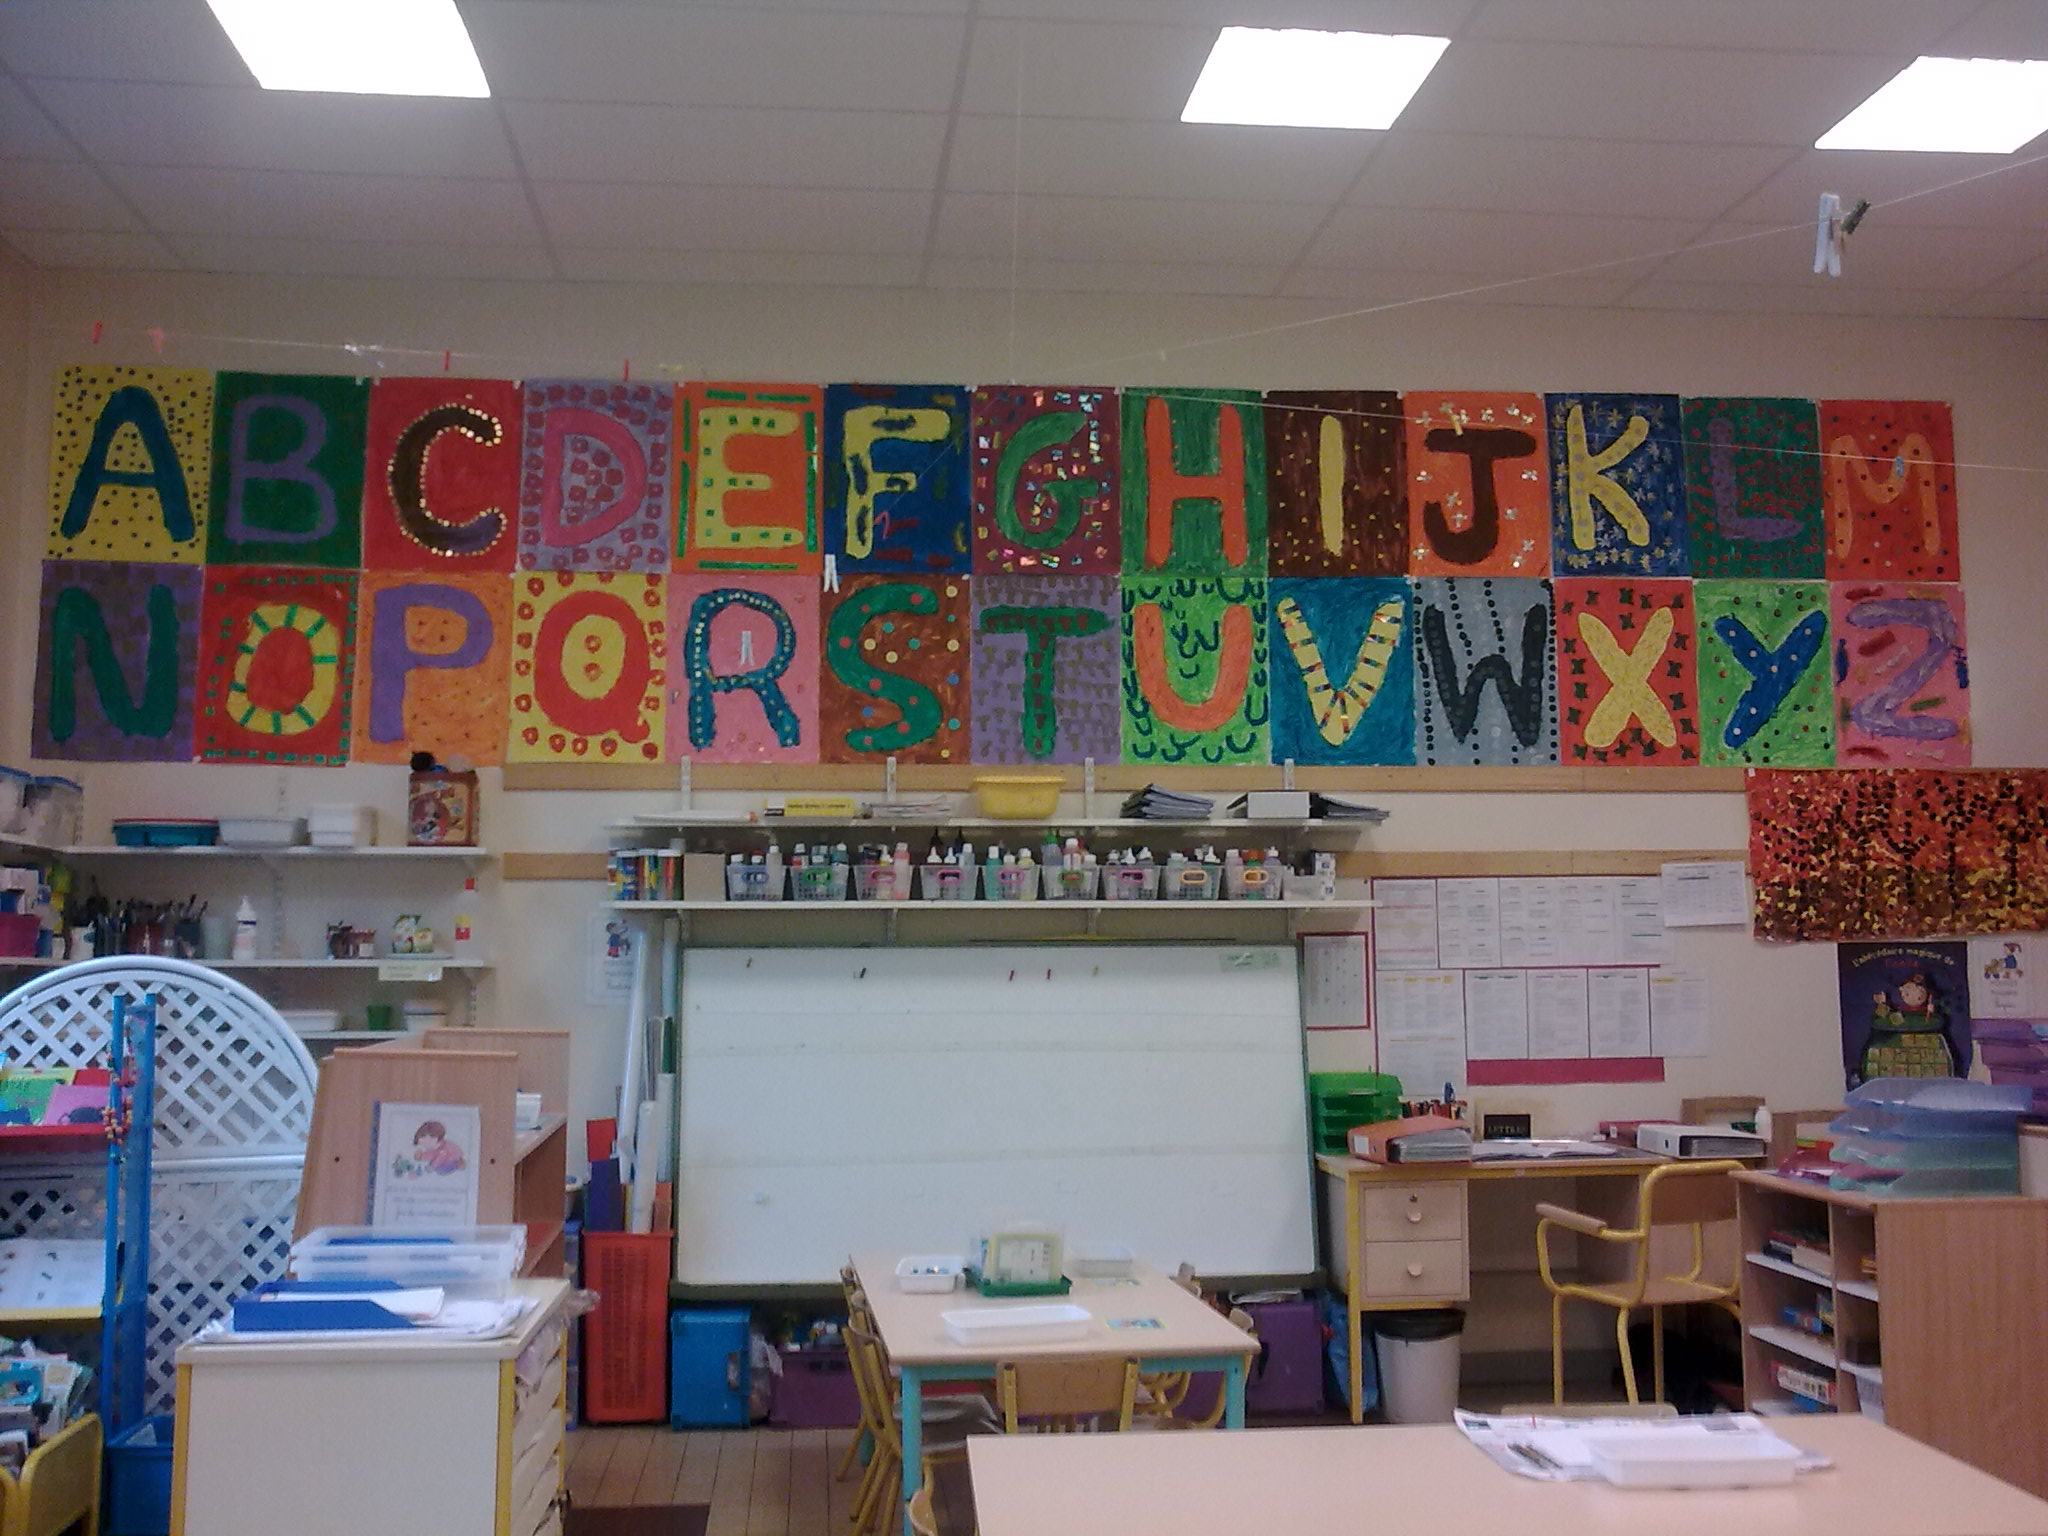
\includegraphics[height = 0.35\textheight]{./fotky/Obr6.jpg}
		\caption{
			Výzdoba třídy písmeny abecedy (viz.~\ref{tridaVybaveni}).
		}
		\label{Obr6}
	\end{figure}


	\begin{figure}[tb]
		\centering
		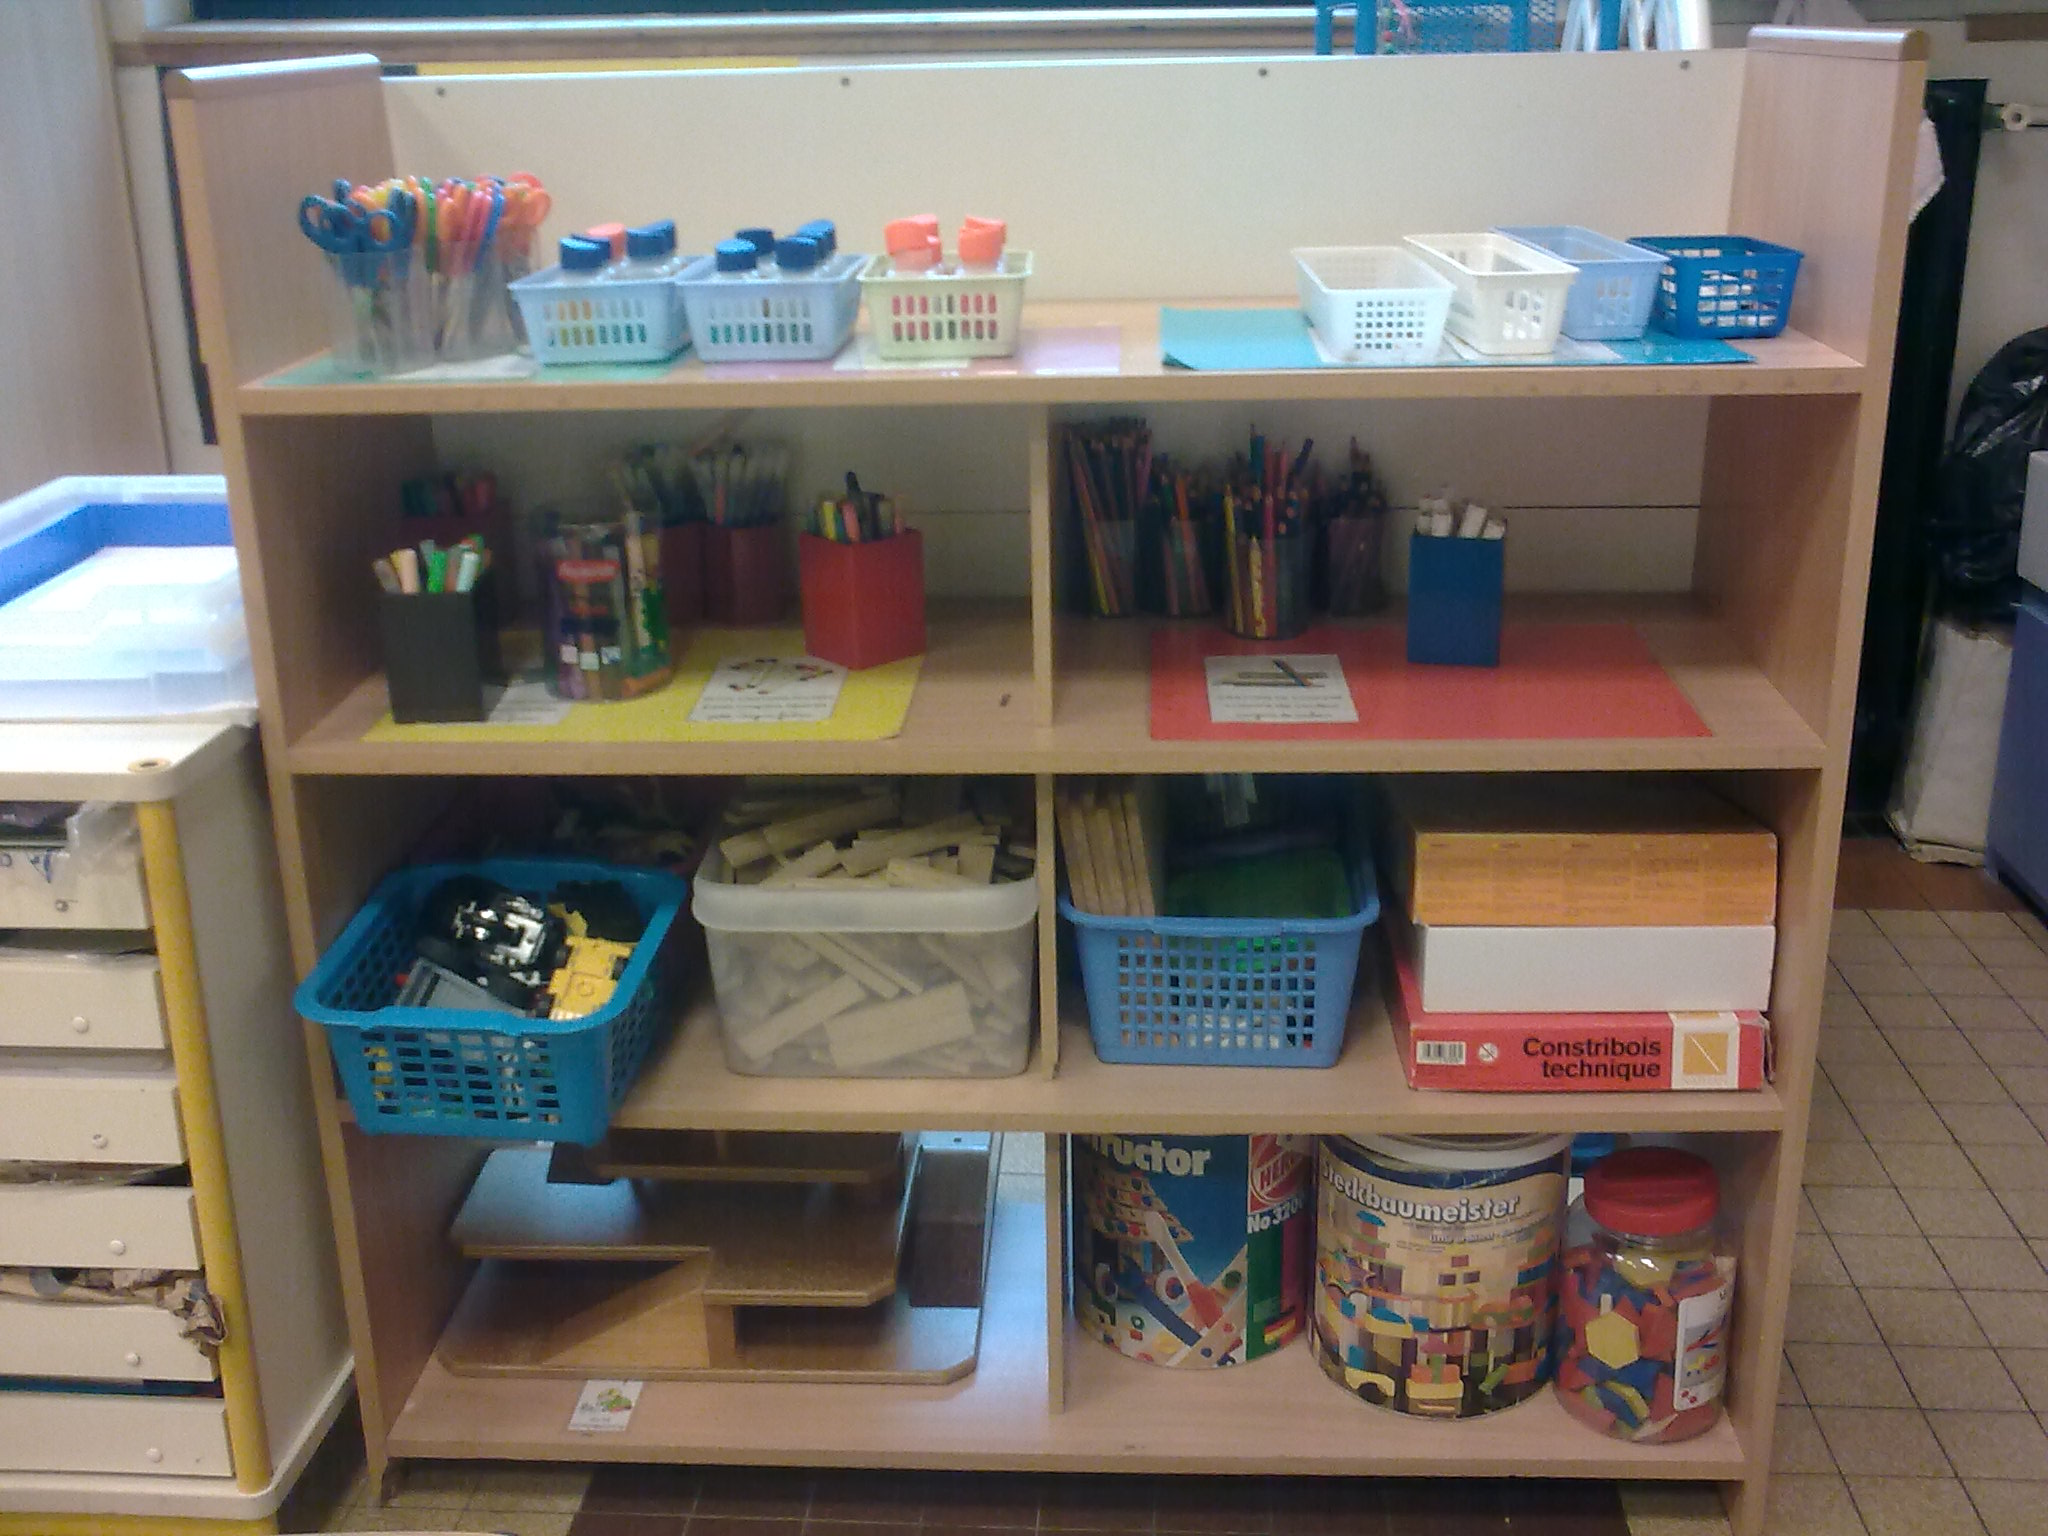
\includegraphics[height = 0.35\textheight]{./fotky/Obr7.jpg}
		\caption{
			Police na materiál a pomůcky (viz.~\ref{tridaVybaveni}).
		}
		\label{Obr7}
	\end{figure}

	\begin{figure}[tb]
		\centering
		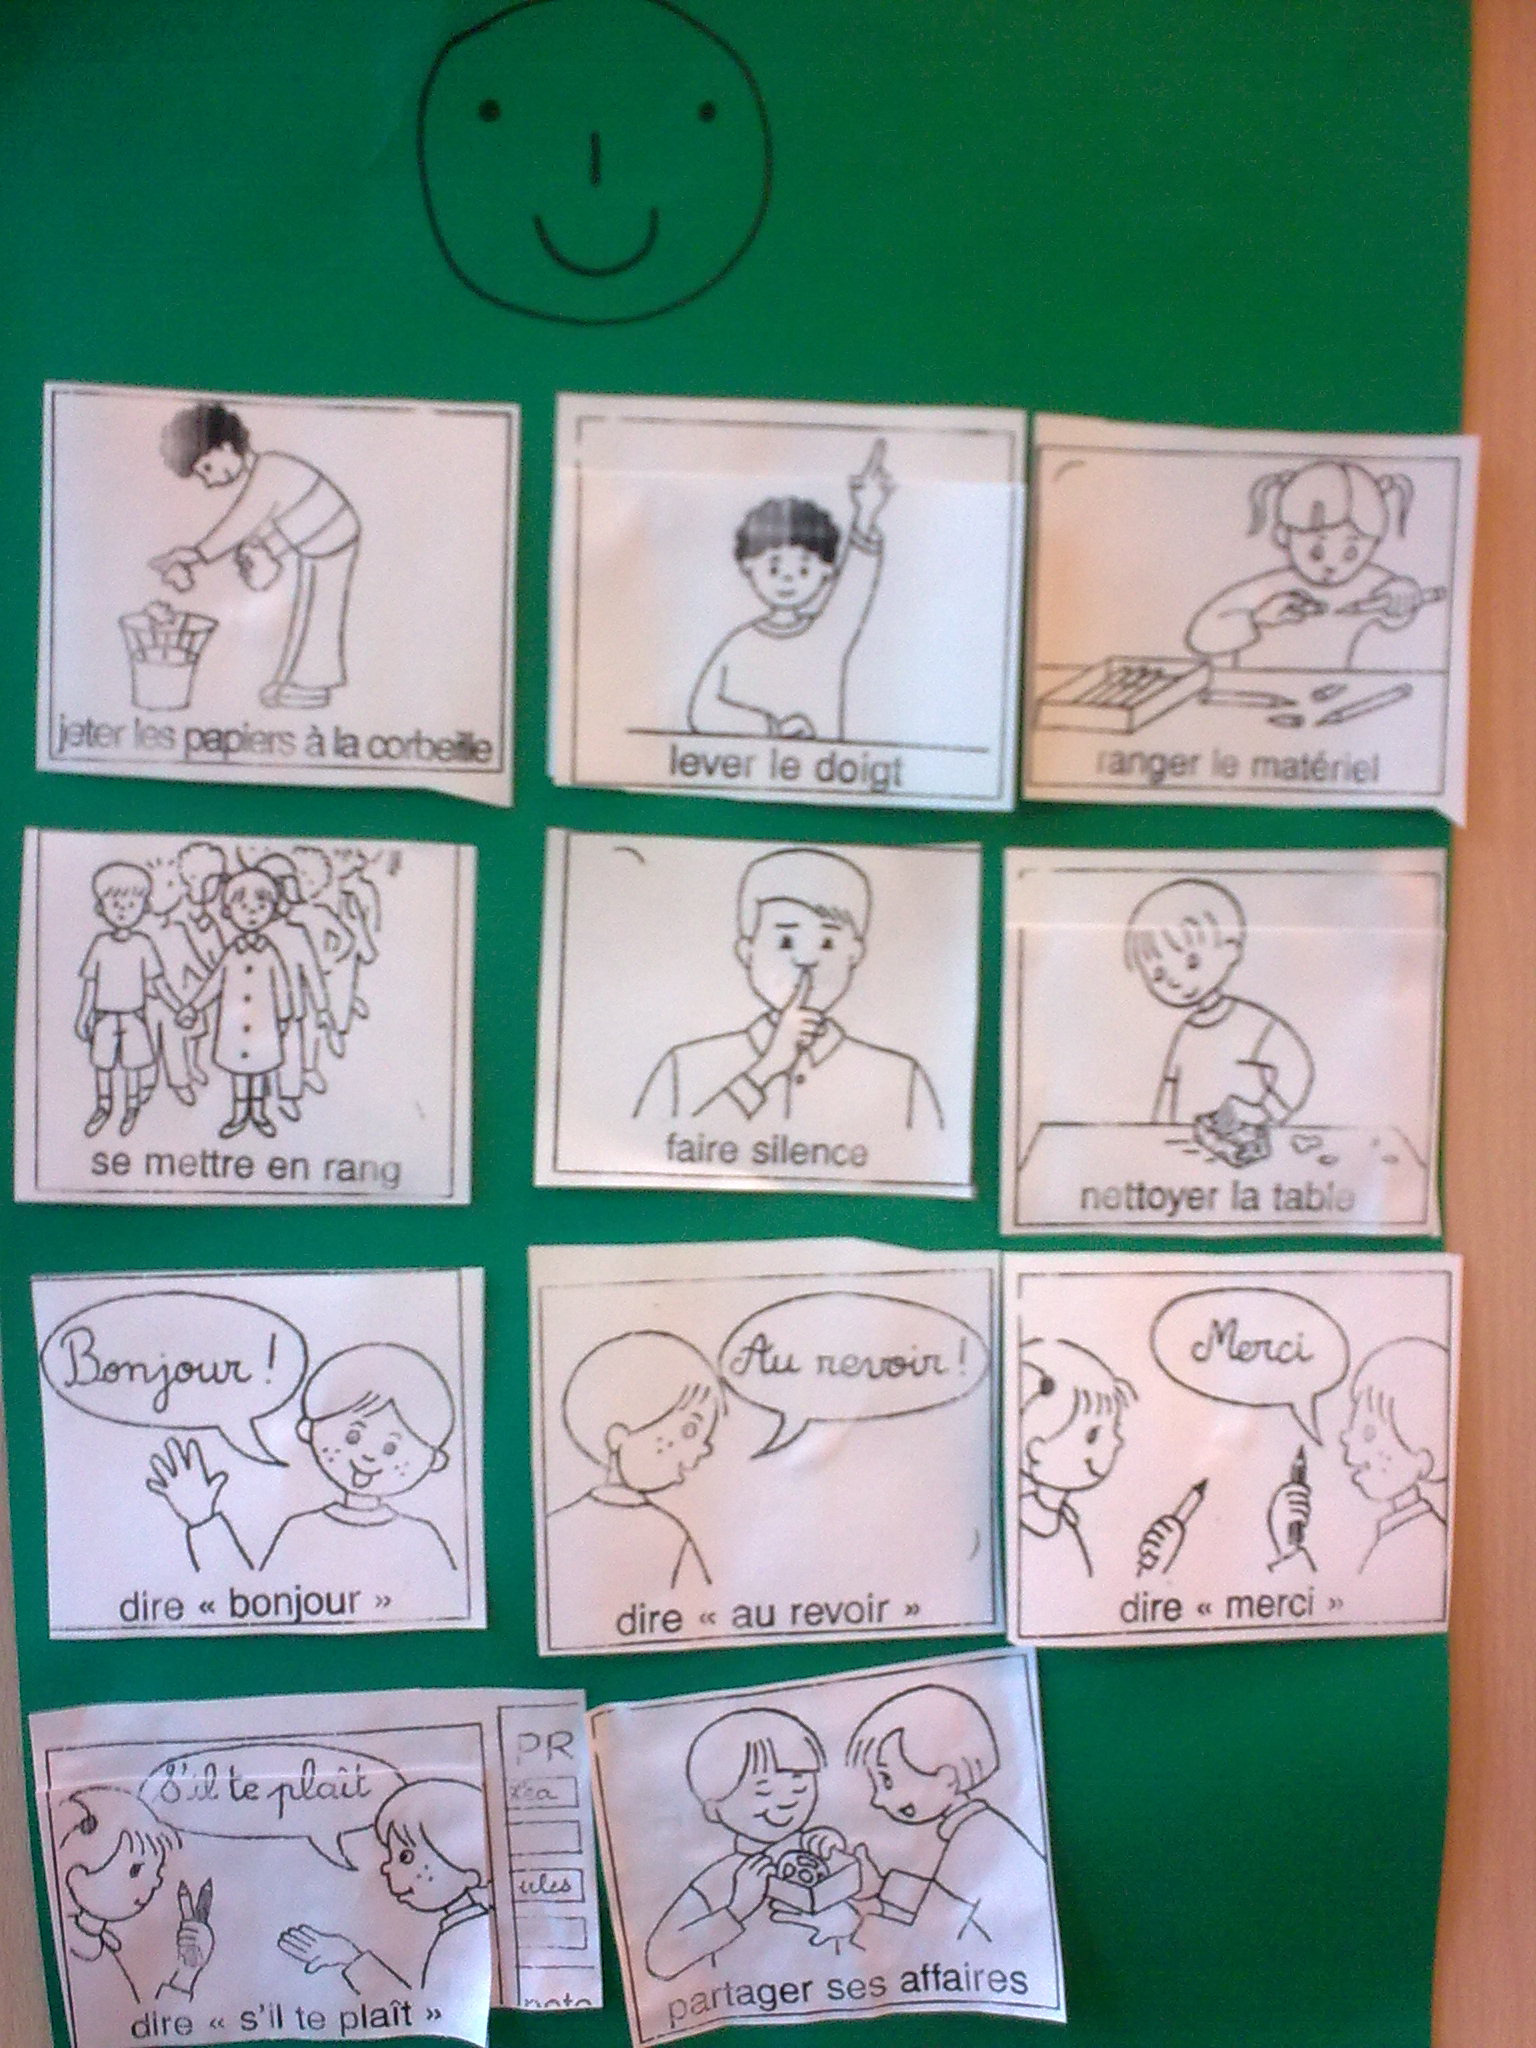
\includegraphics[width = 0.45\linewidth]{./fotky/Obr8a.jpg}
		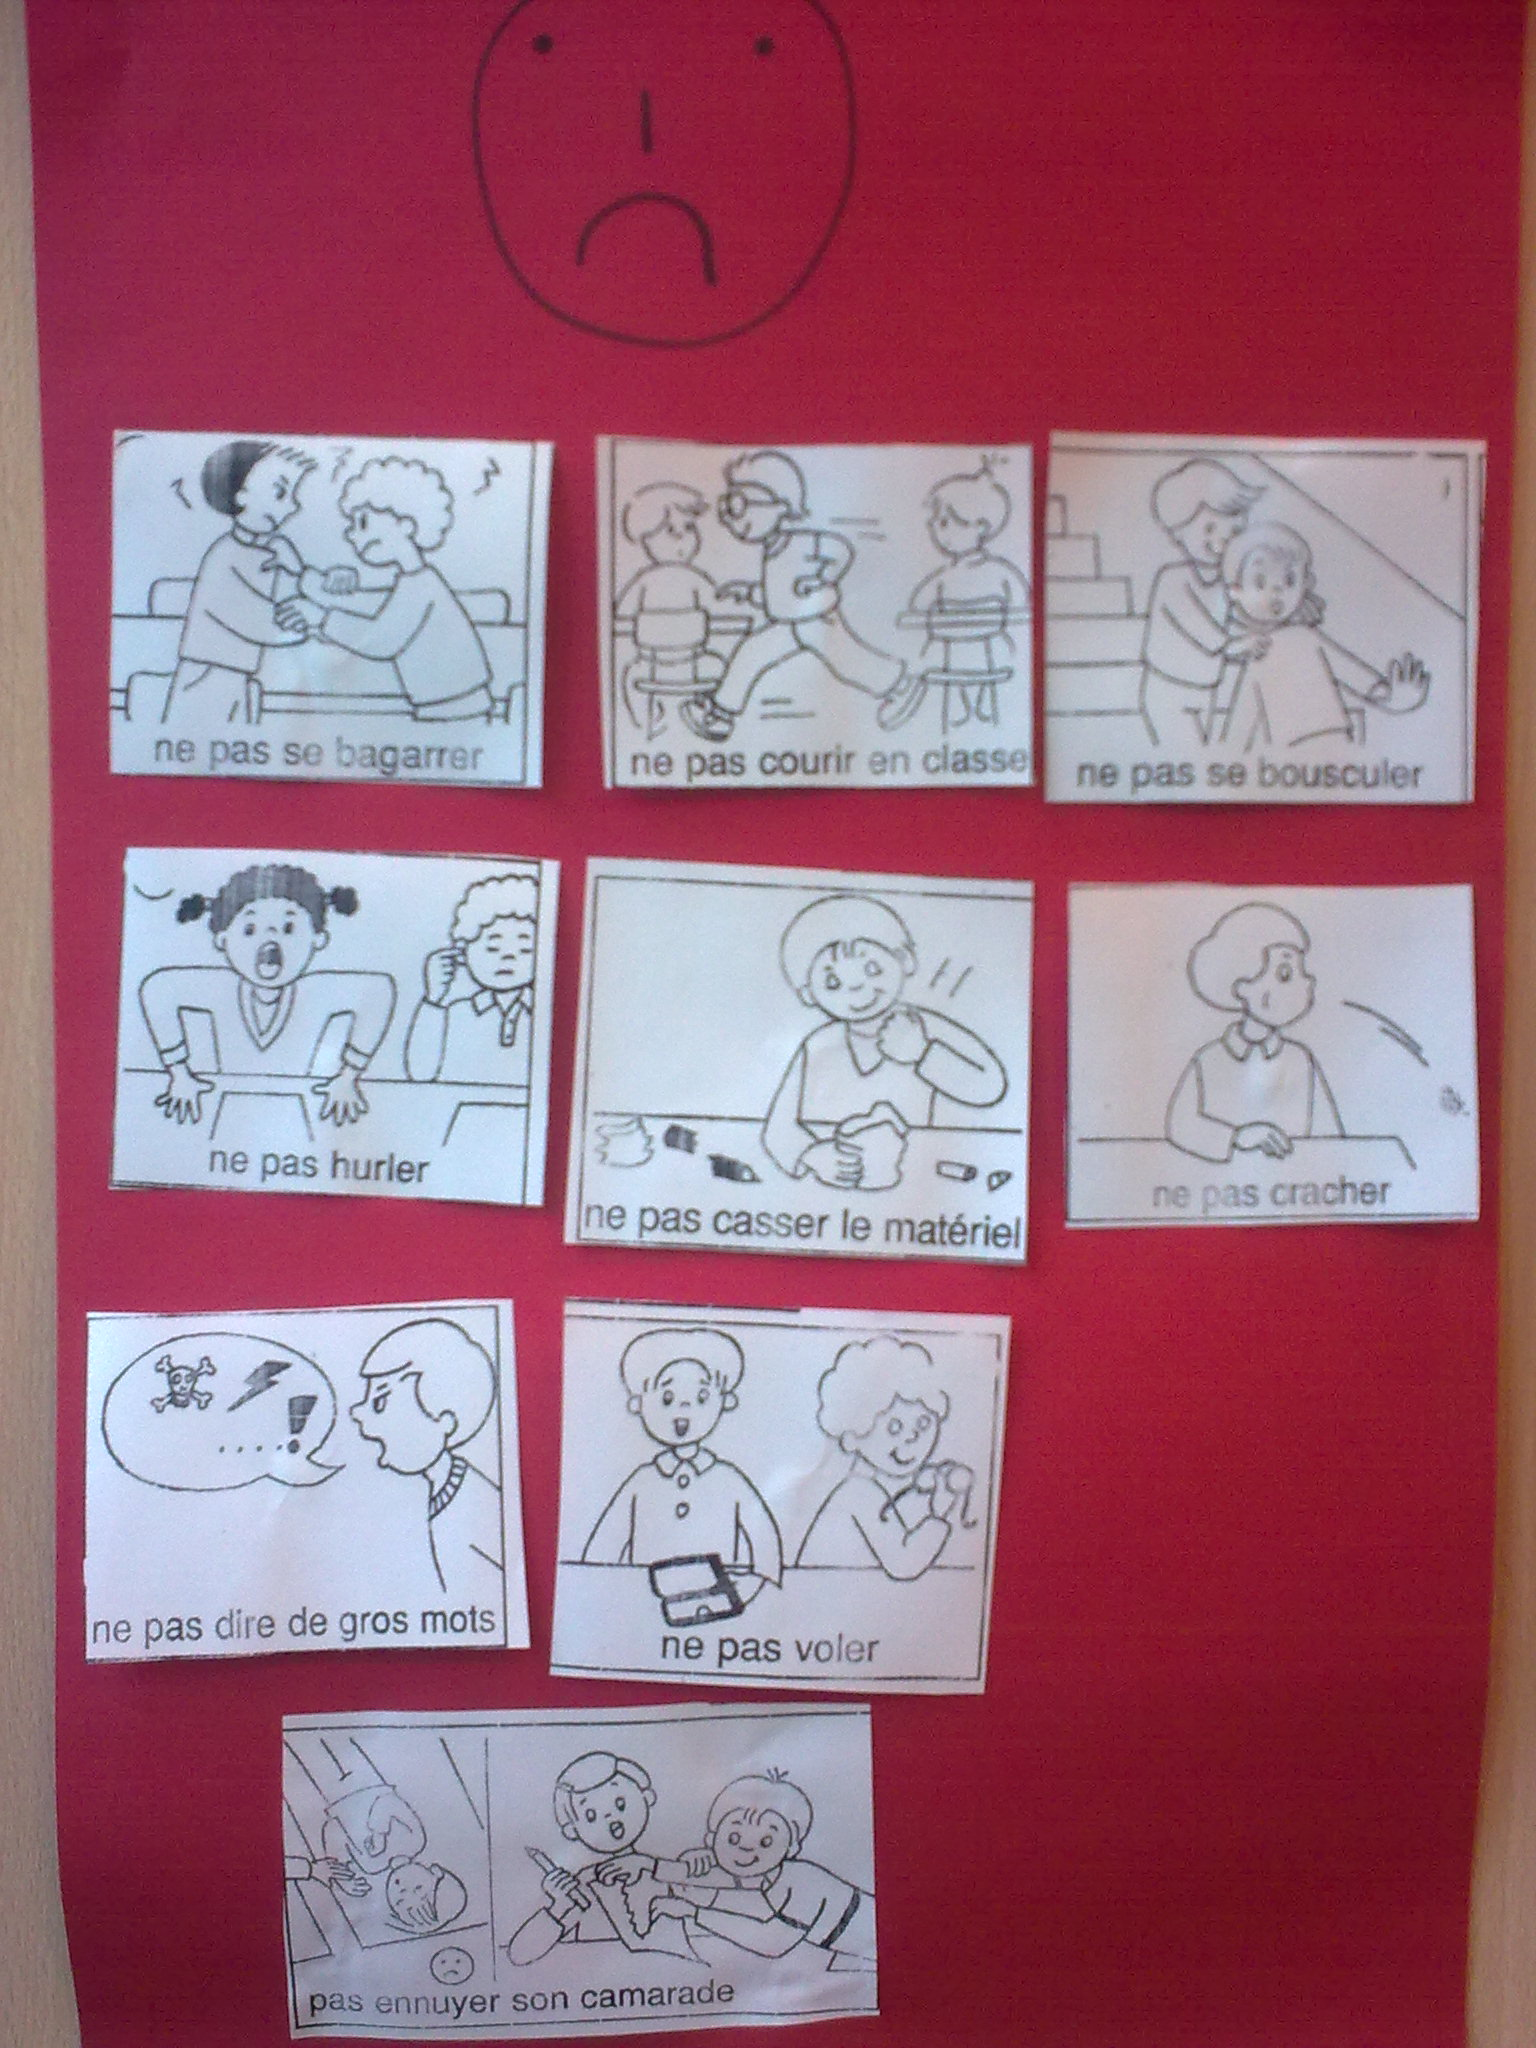
\includegraphics[width = 0.45\linewidth]{./fotky/Obr8b.jpg}
		\caption{
			Vyvěšená pravidla třídy (viz.~\ref{pravidlaChovani}).
		}
		\label{Obr8}
	\end{figure}

	\begin{figure}[tb]
		\centering
		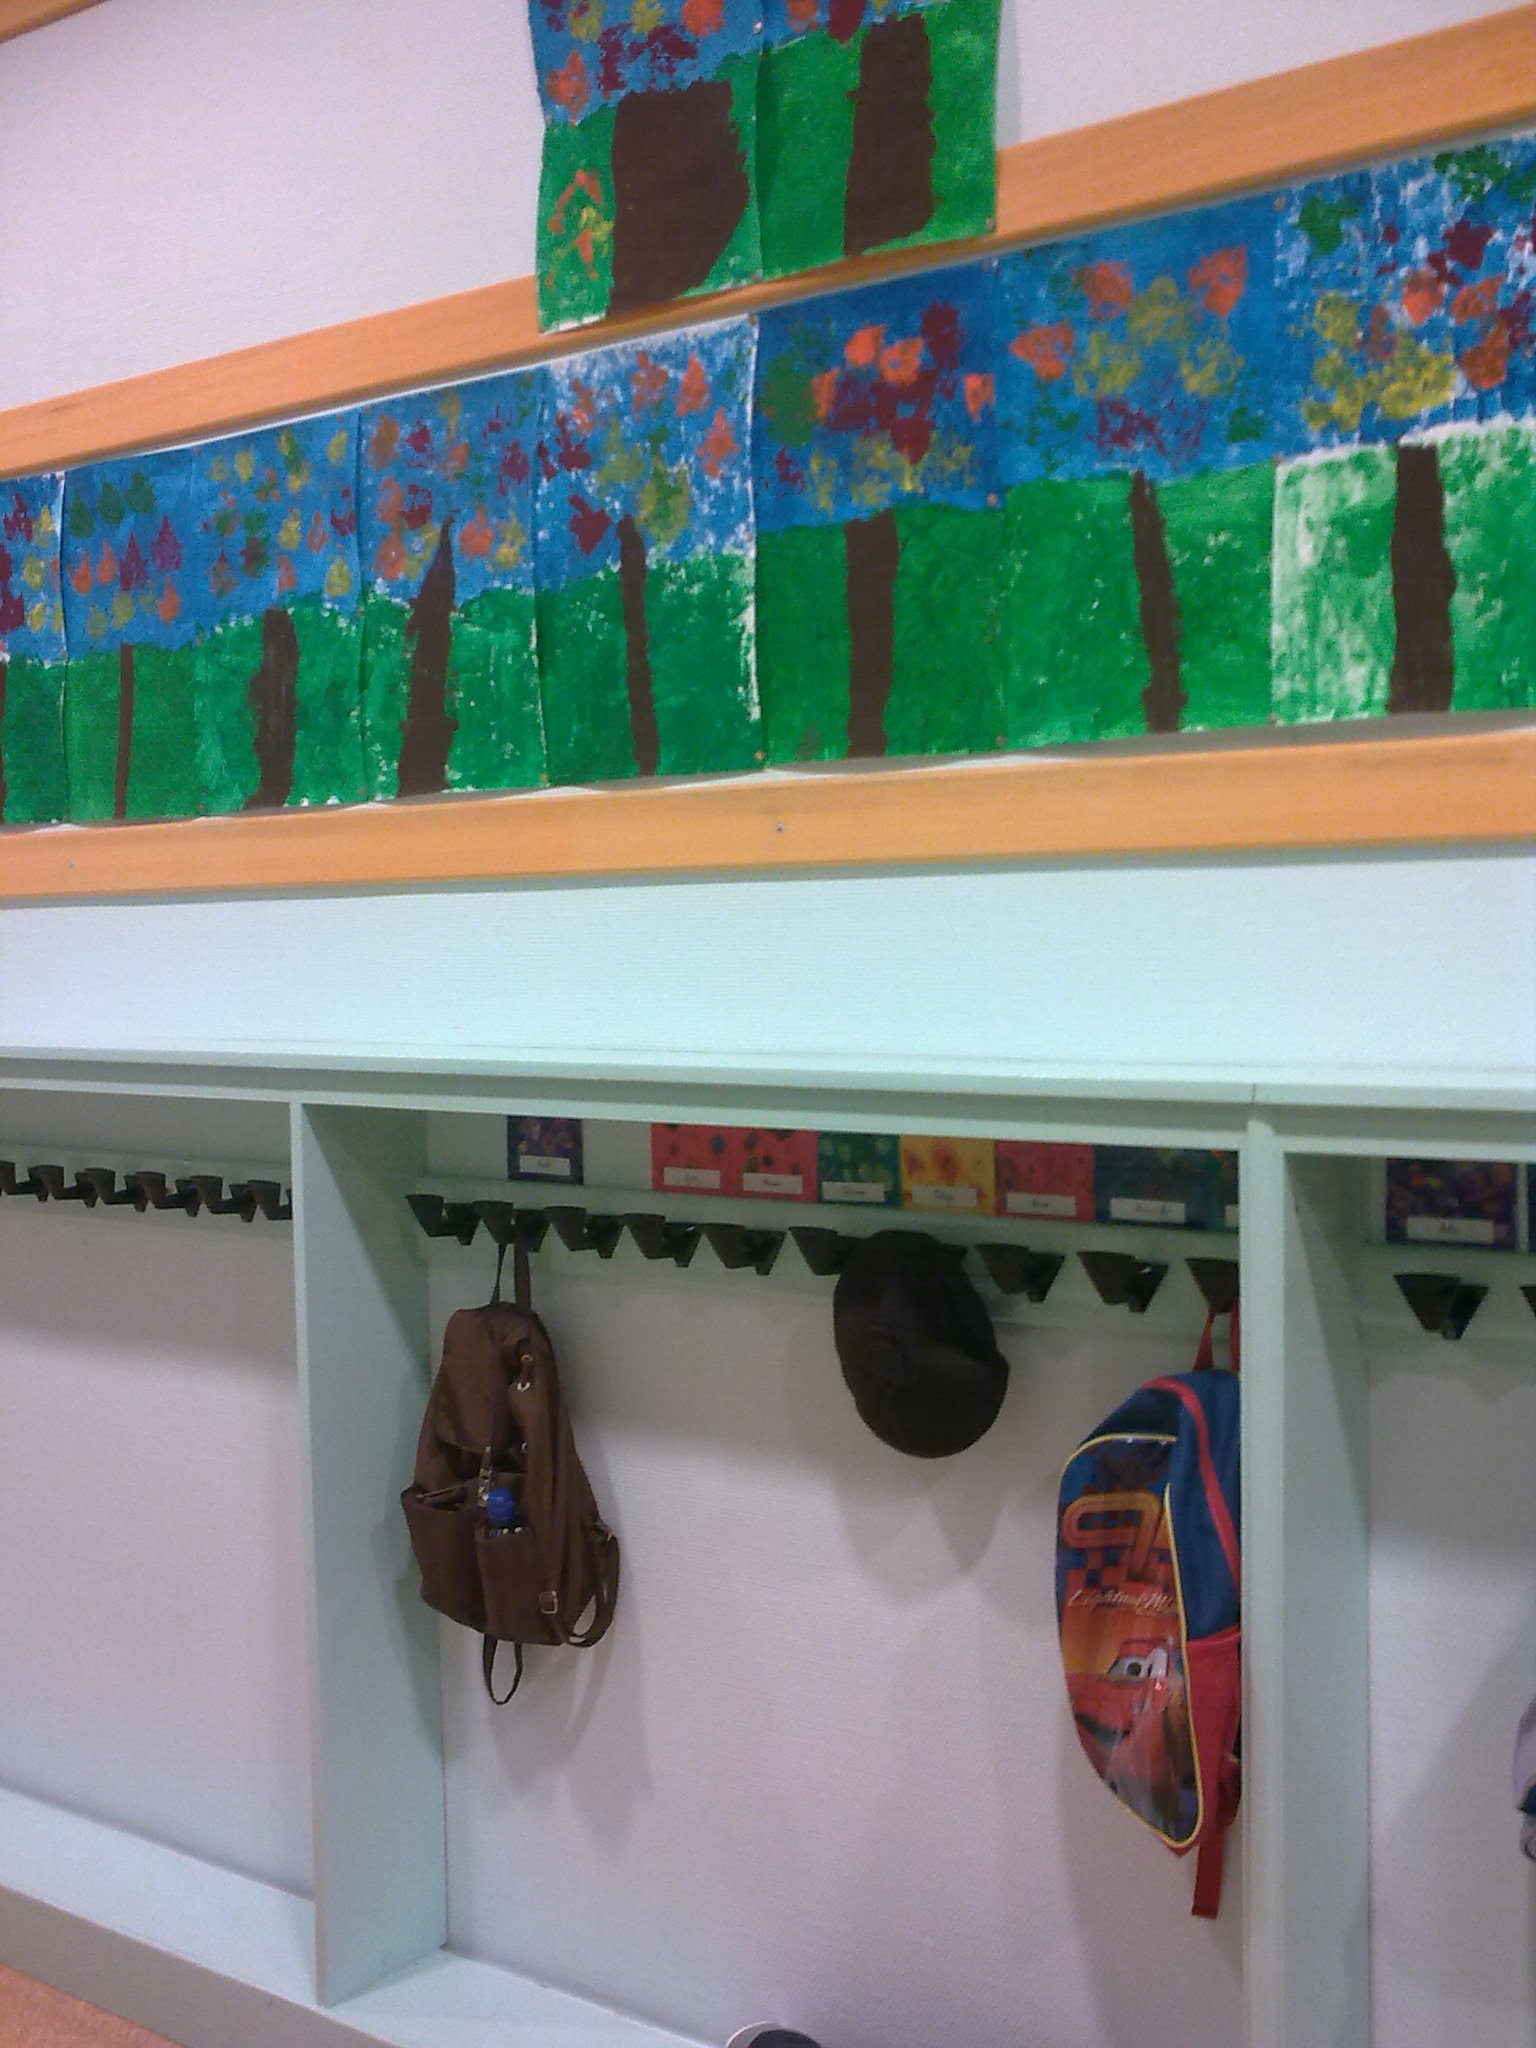
\includegraphics[height = 0.35\textheight]{./fotky/Obr9.jpg}
		\caption{
			Šatna (viz.~\ref{prichod}).
		}
		\label{Obr9}
	\end{figure}


